\section{Variational Autoencoder}\raggedbottom
\label{vae}
Variational Autoencoder \citep{kingma2014autoencoding} gehören zu den probabilistischen generativen Modellarchitekturen. In den letzten Jahren haben generative Modelle, insbesondere auch Variational Autoencoder, beeindruckende Möglichkeiten aufgezeigt, hochrealistische Daten wie zum Beispiel Bilder, Texte oder Audios zu generieren.
Generative Modelle versuchen die Merkmale und Verteilung eines Datensatzes zu verstehen und anschließend neuartige Datenbeispiele, die ähnlich zum Trainingsdatensatz sind zu generieren.

Autoencoder sind neuronale Netze, die trainiert werden, um Eingabedaten zu komprimieren und anschließend zu rekonstruieren. 
Sie bestehen aus einem Encoder $\mathbf{E}:\mathbb{R}^n \rightarrow \mathbb{R}^m$ und einem Decoder $\mathbf{D}:\mathbb{R}^m \rightarrow \mathbb{R}^n$, wobei der Encoder versucht, eine komprimierte Darstellung $c \in \mathbb{R}^{m}$ für die Eingabedaten $x \in \mathbb{R}^{n}$ im Latentspace zu finden. Die komprimierte Darstellung im Latentspace wird vom Decoder rekonstruiert mit dem Ziel, eine möglichst identische Rekonstruktion zur Eingabe $x \in \mathbb{R}^{n}$ zu erzeugen.
Um stets eine komprimierte Darstellung im Latentraum zu erhalten und nicht eine Identitätsabbildung für den Encoder und Decoder wird die Dimension der Latentrepräsentation niederiger als die Eingabedimension gewählt, also $m<n$ \citep{introVAE}. 

Da Autoencoder nur einen diskreten Latentraum erzeugen existieren im Latentraum viele leere Stellen, wodurch Interpolation durch den Latentraum zur Rekonstruktion neuer Ausgaben kaum möglich ist.
%Autoencoder erzeugen nur einen diskreten Latentraum, wodurch Interpolation durch den Latentraum zur Rekonstruktion neuer Ausgaben kaum möglich ist, da im Latentraum viele leere Stellen existieren. 
Dies ist darauf zurückzuführen, dass ein Autoencoder auf möglichst geringen Verlust beim Encodieren und Decodieren trainiert wird und somit keinen Wert auf die Organisation des Latentraums legt. 
%Somit führt die fehlende Regularisierung der einzelnen Datenpunkte oft zu Overfitting.


\begin{figure}[h]
    \centering
    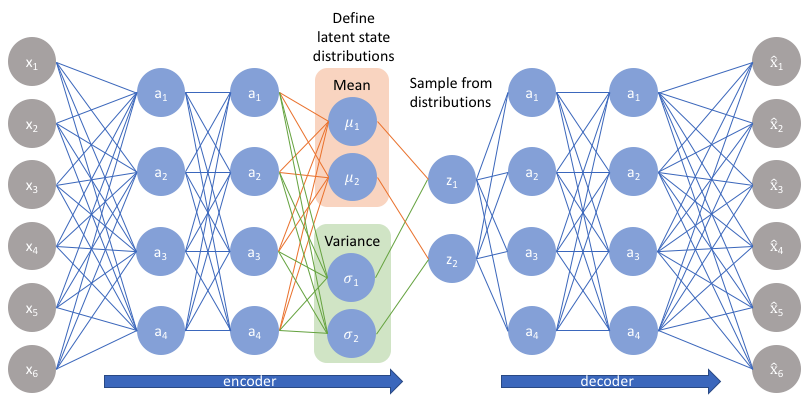
\includegraphics[width=12cm]{bilder/vae}
    \caption{VAE Modellarchitektur \citep{jordan_2018}}
    \label{vae_model}
\end{figure}

Im Gegensatz zu Autoencodern verwenden Variational Autoencoder einen probabilistischen Ansatz, um Datenpunkte $x_i$ eines Datensatzes $X$, der durch die unbekannte Wahrscheinlichkeitsfunktion $P(\mathbf{X})$ beschrieben wird, im Latentraum $Z$ zu repräsentieren. 
Die Architektur und der probabilistische Ansatz wird in Abbildung \ref{vae_model} dargestellt.
Für den Datensatz $X$ mit Datenpunkten $x_i$ wird angenommen, dass ein generatives Modell mit den Parametern $\theta$ existiert, welches mittels Latentvektor $z_i$ diesen Datenpunkt $x_i$ generieren kann.

%only for pagebreak
Dieser generative Teil des Variational Autoencoders ist der Decoder des  Netzes, welcher approximativ versucht, die Daten als Verteilung $p_\theta (\mathbf{x})$ zu modellieren.
\begin{equation}
    \label{px}
p_\theta (\mathbf{x}) = \int_{\mathbf{z}} p_\theta (\mathbf{x\mid z}) p_\theta (\mathbf{z}) dz
\end{equation}
In Gleichung \ref{px} wird für $p_\theta (\mathbf{z})$ die A-priori-Wahrscheinlichkeit angenommen und für $p_\theta (\mathbf{x\mid z})$ die Likelihood. Der Decoder zieht demnach eine Latentvariable $z$ aus der A-priori-Menge $p_\theta (\mathbf{z})$ und berechnet mit der Likelihood $p_\theta (\mathbf{x\mid z})$ Datenpunkte $x$ \citep{vae2}.

Die inferierten Latentvariablen für die bekannten Datenpunkte $X$ lassen sich über die A-posteriori-Wahrscheinlichkeit $p_\theta (\mathbf{z\mid x})$ aus Gleichung \ref{posteriori} herleiten. 

\begin{equation}
    \label{posteriori}
    p_\theta (\mathbf{z\mid x}) = \frac{p_\theta (\mathbf{x\mid z}) p_\theta (\mathbf{z})}{p_\theta(\mathbf{x})}
\end{equation}

%Die Berechnung von $p_\theta(x)$ ist meistens nicht möglich. Demnach lässt sich auch $p_\theta (z|x)$ nicht trivial berechnen. 
Der Encoder des Variational Autoencoder approximiert die A-posteriori-Wahrscheinlichkeit durch ein Inferenzmodell $q_\phi (\mathbf{z\mid x})$, da sich $p_\theta (\mathbf{z\mid x})$ nicht trivial berechnen lässt.
Die Parameter $\phi$ des Encoders werden optimiert, um mit $q_\phi (\mathbf{z\mid x}) \approx p_\theta (\mathbf{z\mid x})$ die wahre A-posteriori-Verteilung zu approximieren, indem die Kullback-Leibler-Divigenz zwischen den beiden Wahrscheinlichkeiten minimiert wird, wie in Abschnitt \ref{elbo} beschrieben.



% Der Encoder des Variational Autoencoder encodiert die Eingaben in jeweils eine multivariate Verteilung von der anschließend Latentvektoren $z_i$ gezogen werden. 
% Die Latentvektoren werden anschließend vom Decoder decodiert und der Rekonstruktionsfehler zurückgegeben.
% %Normalerweise werden für die Encodierteverteilung 
% %Normalverteilung Regalusierung erklären https://towardsdatascience.com/understanding-variational-autoencoders-vaes-f70510919f73




% Die Beziehungen zwischen den Eingabedaten $x$ und den Latentvektoren $z$ sind wie folgt definiert, wobei $\phi$ die Parameter des Encoders und $\theta$ die Parameter des Decoders sind:
% \begin{itemize}
% \item Prior $p_\theta (z)$
% \item Likelihood $p_\theta (x|z)$
% \item Posterior $p_\theta (z|x)  \approx q_\phi (z|x)$
% \end{itemize}
% %ANDERS AUFSCHREIBEN

% Da die Posterior Verteilung $p_\theta (z|x)$ nicht bestimmt werden kann, approximieren wir diese mit $q_\phi (z|x)$ unter Verwendung der Variationsinferenzmethode zur Minimierung der Kullback-Leibler-Divergenz, wie in Abschnitt \ref{elbo} beschrieben.

% Um mittels Variational Autoencoder neue Datenobjekte zu samplen wird zunächst mit der Prior-Verteilung $p_\theta (z)$ ein neuer Latentvektor $\hat{z}$ gezogen. Anschließend lässt sich ein neues Datenobjekt $\hat{x}$ mit der Verteilung $p_\theta (x|z=\hat{z})$ generieren.
\subsection{Evidence Lower Bound}
%https://lilianweng.github.io/lil-log/2018/08/12/from-autoencoder-to-beta-vae.html#contractive-autoencoder
%https://openreview.net/forum?id=Sy2fzU9gl
%https://arxiv.org/pdf/1312.6114.pdf
%http://mediatum.ub.tum.de/doc/1547089/1547089.pdf
%https://pub.tik.ee.ethz.ch/students/2018-FS/MA-2018-22.pdf
%https://mediatum.ub.tum.de/doc/1547089/file.pdf
%https://www.jeremyjordan.me/variational-autoencoders/
%https://towardsdatascience.com/understanding-variational-autoencoders-vaes-f70510919f73
%https://arxiv.org/pdf/1906.02691.pdf
%https://arxiv.org/pdf/1903.10145.pdf
%https://ichi.pro/de/generative-modellierung-mit-variational-auto-encoder-vae-277371603749134
%https://xyang35.github.io/2017/04/14/variational-lower-bound/

\label{elbo}
Die Lossfunktion von Variational Autoencodern ist die \textbf{E}vidence \textbf{L}ower \textbf{Bo}und (ELBO).
Bei Variational Autoencodern ist das Optimierungsziel die gleichzeitige Minimierung des Rekonstruktionsfehlers des generativen Modells $\theta$ zwischen Eingabe- und Ausgabedaten sowie die Approximation von $p_\theta (\mathbf{z\mid x})$ mit $q_\phi (\mathbf{z\mid x})$ durch Minimierung der Kullback-Leibler-Divergenz$D_{KL}(q_\phi(\mathbf{z\mid x})\parallel p_\theta(\mathbf{z\mid x}))$.
Für eine beliebige Wahl der Decoder Parameter $\phi$ gilt \citep{introVAE}:
\begin{align}
    log(p_\theta(\mathbf{x})) &= \mathbb{E}_{ q_\phi(\mathbf{z\mid x}) } [log( p_\theta(\mathbf{x}) )] \nonumber \\
    &= \mathbb{E}_{q_\phi( \mathbf{z\mid x} )} \Bigl[ log \Bigl[ \tfrac{ p_\theta(\mathbf{x,z}) }{ p_\theta(\mathbf{z \mid x}) } \Bigr] \Bigr] \nonumber \\
    &= \mathbb{E}_{q_\phi( \mathbf{z\mid x} )} \Bigl[ log \Bigl[ \tfrac{ p_\theta(\mathbf{x,z}) }{ q_\phi( \mathbf{z\mid x} ) } \tfrac{ q_\phi( \mathbf{z\mid x} ) }{ p_\theta(\mathbf{z \mid x}) }\Bigr] \Bigr] \nonumber \\
    &= \underbrace{\mathbb{E}_{q_\phi( \mathbf{z\mid x} )} \Bigl[ log \Bigl[ \tfrac{ p_\theta(\mathbf{x,z}) }{ q_\phi( \mathbf{z\mid x} ) } \Bigr] \Bigr]}_{=\mathcal{L}_{\theta,\phi}(\mathbf{x}) \text{ (ELBO)}} + \underbrace{\mathbb{E}_{q_\phi( \mathbf{z\mid x} )} \Bigl[ log \Bigl[ \tfrac{ q_\phi( \mathbf{z\mid x} ) }{ p_\theta(\mathbf{z \mid x}) }\Bigr] \Bigr]}_{=D_{KL}(q_\phi(\mathbf{z\mid x})\parallel p_\theta(\mathbf{z\mid x}))} \label{elbo4}
\end{align}
In Zeile \ref{elbo4} ist der erste Term die Evidence Lower Bound und der zweite Teil die Kullback-Leibler Divergenz.
Die Kullback-Leibler Divergenz zwischen $q_\phi(\mathbf{z\mid x})$ und $p_\theta(\mathbf{z\mid x})$ ist nicht negativ und genau null, wenn $q_\phi(\mathbf{z\mid x})$ der wahren A-posteriori-Verteilung entspricht.

\begin{equation}
    \label{dkl}
    D_{KL}(q_\phi(\mathbf{z\mid x})\parallel p_\theta(\mathbf{z\mid x})) \geq 0
\end{equation}

Aus Gleichung \ref{elbo4} lässt sich durch Umformung die Evidence Lower Bound Funktion aufstellen:
\begin{equation}
    \label{realelbo}
    \mathcal{L}_{\theta,\phi}(\mathbf{x}) = log(p_\theta(\mathbf{x})) - D_{KL}(q_\phi(\mathbf{z\mid x})\parallel p_\theta(\mathbf{z\mid x})) \leq log(p_\theta(\mathbf{x})) 
\end{equation}
Aufgrund der nicht Negativität der Kullback-Leibler Divergenz in Gleichung \ref{dkl} ist die Evidence Lower Bound eine untere Schranke der Log-Likelihood der Datenmenge.
Bei Maximierung der Evidence Lower Bound Funktion in Gleichung \ref{realelbo} wird die Evidenz $log(p_\theta(\mathbf{x}))$ maximiert, wodurch das generative Modell verbessert wird. Ebenfalls wird die Kullback-Leibler Divergenz minimiert, wodurch der Encoder die A-posteriori-Verteilung besser approximieren kann.

Somit wird als Lossfunktion $\mathbf{L}_{\theta,\phi}$ die negative Evidence Lower Bound Funktion gewählt, die es zu minimieren gilt:
\begin{align}
    \mathbf{L}_{\theta,\phi} &= -\mathcal{L}_{\theta,\phi}(\mathbf{x}) = -log(p_\theta(\mathbf{x})) + D_{KL}(q_\phi(\mathbf{z\mid x})\parallel p_\theta(\mathbf{z\mid x}))  \\
    \hat{\theta},\hat{\phi} &= \underset{\theta, \phi}{\arg\min \ } \mathbf{L}_{\theta,\phi}
\end{align}
Diese Lossfunktion erlaubt das simultane Optimieren der beiden Parameter $\theta$ und $\phi$.


% \begin{align*}
%     \small
%     D_{KL}(q_\phi(\mathbf{z\mid x})\parallel p_\theta(\mathbf{z\mid x})) &= \int q_\phi(\mathbf{z\mid x}) \log \frac{q_\phi(\mathbf{z\mid x})}{p_\theta(\mathbf{z\mid x})} \, d\mathbf{z}\\
%     &= \int q_\phi(\mathbf{z\mid x}) \log \frac{q_\phi(\mathbf{z\mid x})p_\theta(\mathbf{x})}{p_\theta(\mathbf{z,x})} \,d\mathbf{z}\\
%     &= \int q_\phi(\mathbf{z\mid x}) \left( \log (p_\theta(\mathbf{x})) + \log \frac{q_\phi(\mathbf{z\mid x})}{p_\theta(\mathbf{z,x})}\right) d\mathbf{z}\\
%     &= \log (p_\theta(\mathbf{x})) + \int q_\phi(\mathbf{z\mid x}) \log \frac{q_\phi(\mathbf{z\mid x})}{p_\theta(\mathbf{z,x})} \,d\mathbf{z}\\
%     &= \log (p_\theta(\mathbf{x})) + \int q_\phi(\mathbf{z\mid x}) \log \frac{q_\phi(\mathbf{z\mid x})}{p_\theta(\mathbf{x\mid z})p_\theta(\mathbf{z})} \,d\mathbf{z}\\
%     &= \log (p_\theta(\mathbf{x})) + E_{\mathbf{z} \sim q_\phi(\mathbf{z\mid x})}(\log \frac{q_\phi(\mathbf{z\mid x})}{p_\theta(\mathbf{z})} - \log(p_\theta(\mathbf{x\mid z})))\\
%     &= \log (p_\theta(\mathbf{x})) + D_{KL}(q_\phi(\mathbf{z\mid x}) \parallel p_\theta(\mathbf{z})) - E_{\mathbf{z} \sim q_\phi(\mathbf{z\mid x})}(\log(p_\theta(\mathbf{x\mid z})))
% \end{align*}
% der \textbf{E}vidence \textbf{L}ower \textbf{B}ound (ELBO).


% ÜBERARBEITEN
\subsubsection{Reparametisierung} %kingma welling
Zum Training des Variational Autoencoder wird mittels Backpropagation der Fehler des Netzwerkes propagiert. Da das Samplen von $z \sim q_\phi(\mathbf{z\mid x})$ nicht deterministisch ist, kann hier keine Backpropagation durchgeführt werden.
Um dennoch Backpropagation verwenden zu können wird mittels Reparametisierung $z$ durch eine deterministische Funktion $z=f_\phi(x,\epsilon)$ dargestellt mit $\epsilon$ als externe unabhängige Hilfsvariable \citep{kingma2014autoencoding,jordan_2018}. 
Bei einer multivariaten Gaussverteilung für $q_\phi (\mathbf{z\mid x})$ wäre die Reparametisierung wie folgt, wobei $\times$ die elementweise Multiplikation denotiert:
\begin{align}
    \mathbf{z} \sim q_\phi(\mathbf{z\mid x}) = \mathcal{N}(\mathbf{z;\mu,\sigma \mathcal{I}}) \nonumber \\
    \mathbf{z} = \mu + \sigma \times \mathbf{\epsilon} \text{ , mit } \mathbf{\epsilon} \sim \mathcal{N}(0,\mathcal{I}) 
\end{align}

\subsection{Cyclical Annealing Schedule}
\label{cyc_anneal}
Trainieren von Variational Autoencodern als Sprachmodell im Bereich des Natural Language Processing ist aufgrund des KL-Vanishing Problems besonders schwierig.
VAE Sprachmodelle sollen bei der Textgeneration den lokalen Kontext, allerdings auch globale Eigenschaften wie zum Beispiel Thema, Sprachstil oder Stimmung beachten. 
Trotzdem werden von VAE Modellen bei der Generierung oft die globalen Eigenschaften vernachlässigt \citep{cyc_anneal}. 
Dieses Problem ist als KL-Vanishing bekannt, da die KL-Regularisierung des Loss-Terms beim Trainieren von autoregressiven Decodern innerhalb von VAE Sprachmodellen sehr klein wird.
Somit sind die erlernten Features nahezu identisch zu der vorher angenommenen Normalverteilung und der Decoder nutzt keine Latentfeatures bei der Generation. %https://www.microsoft.com/en-us/research/blog/less-pain-more-gain-a-simple-method-for-vae-training-with-less-of-that-kl-vanishing-agony/ nochmal checken

Abhilfe schafft die Verwendung eines $\beta$-Variational Autoencoder \citep{cyc_anneal} mit zyklischem Erhöhen des $\beta$ Wertes.
$\beta$-Variational Autoencoder sind Variational Autoencoder, die mit einen Lagrangemultiplikator $\beta$ die KL-Divergenz der Loss-Funktion gewichten, um besser separierte Latentfaktoren zu finden.
\begin{equation}
    \mathbf{L}_{\beta} (\beta,\theta,\phi)= -\mathbb{E}_{z\sim q_\phi(\mathbf{z\mid x})}[log p_\theta (\mathbf{x\mid z})]- \beta D_{KL}(q_\phi(\mathbf{z\mid x}) \parallel p_\theta(\mathbf{z})) 
\end{equation}
Falls $\beta = 0$ ist wird das Modell wie ein normaler Autoencoder trainiert, bei $\beta = 1$ wie ein normaler Varitional Autoencoder.

Beim zyklischen Erhöhen wird der $\beta$-Wert des VAE während des Trainings monoton von $\beta=0$ auf zum Ende des Trainings $\beta=1$ in kleinen Abständen erhöht.
So kann beim Training des VAE bei $\beta<1$ zunächst der Fokus darauf gelegt werden, mehr Information für die Rekonstruktion zu erlernen. 
Abschließend enthalten bei $\beta=1$ die vorher trainierten $z$ Vektoren bereits mehr Informationen, die zu einer besseren Anpassung als eine zufällige Initialisierung führen.


\subsection{Optimus}
Optimus (\textbf{O}rganizing \textbf{S}entences via \textbf{P}re-trained \textbf{M}odeling of a \textbf{L}atent \textbf{S}pace) \citep{DBLP:journals/corr/abs-2004-04092} ist ein großes vortrainiertes Deep Latent Variable Modell für natürliche Sprache.
Die Modelarchitektur von Optimus ist ein Variational Autoencoder, der als Encoder BERT und als Decoder GPT-2 verwendet wie in Abbildung \ref{optimus_scheme_fig} zu erkennen ist. 
Verwendet wird jeweils das vortrainierte BERT Base Modell $\phi_{BERT}$ und das vortrainierte GPT-2 Base Modell $\theta_{GPT-2}$ beide mit 12 Layern, 12 Attention Heads und einer Hiddensize von 768. 
\begin{figure}[h]
    \centering
    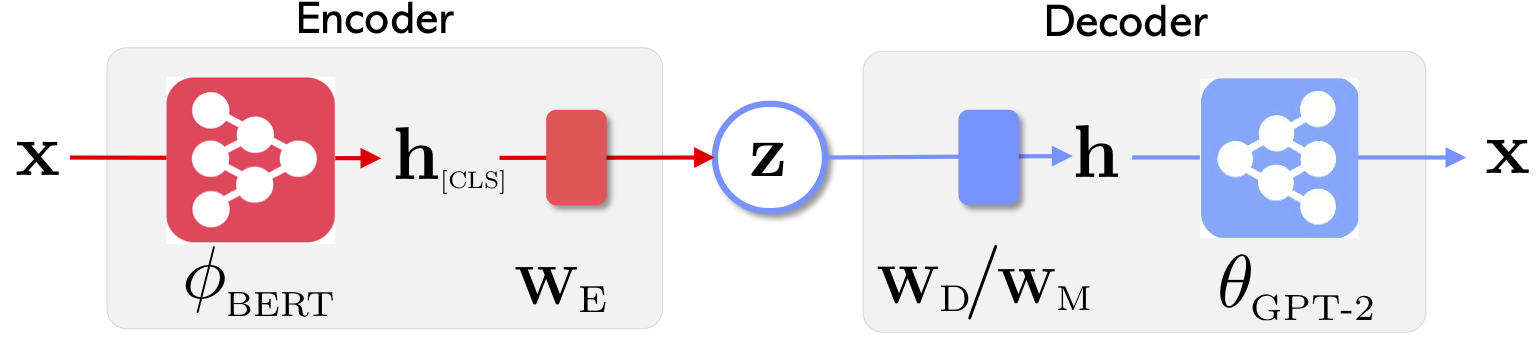
\includegraphics[width=\textwidth]{bilder/optimus_scheme}
    \caption{VAE Modellarchitektur von Optimus mit BERT als Encoder und GPT-2 als Decoder \citep{DBLP:journals/corr/abs-2004-04092}}
    \label{optimus_scheme_fig}
\end{figure}
Trainiert wird Optimus mit dem Ziel, Sätze in einem universellen Latentspace zu organisieren und somit übergreifende semantische Muster für die einzelnen Sätze zu finden.
Somit kann durch gezieltes Verändern des Latentvektors $z$ kontrolliert Text generiert werden. %ÜBERARBEITEN

BERT und GPT-2 über eine VAE Architektur miteinander zu verbinden hat die Herausforderung, die unterschiedlichen Tokenisierungsschemen der einzelnen Modelle zu verwenden und den Latentvektor bei der Textgeneration von GPT-2 zu injizieren. 
Die Eingabetokens von BERT verwenden das WordPiece Embeddings Verfahren \citep{wordpiece} mit einer Vokabulargröße von 28.996 Tokens. 
Die Ausgabe erfolgt über die Byte Pair Encoding Tokenisierung \citep{bytepairencoding} von GPT-2 mit einer Vokabulargröße von 50.260 Tokens. 
Innerhalb des Netzwerkes wird im Latentvektor ein Token durch eine Einbettung $h_{Emb}$, die das Token, die Position und das Segment Embedding wiedergibt, repräsentiert.
Um beim Training den Loss der Rekonstruktionsaufgabe zu berechnen, werden die Sätze mit beiden Tokenisierungen tokenisiert.


Als Latentvektor $z \in \mathbb{R}^P$ wird die gepoolte Ausgabe des letzten Hiddenlayers $h_{[CLS]} \in \mathbb{R}^H$ von BERT mit einer Gewichtsmatrix multipliziert $W_{E} \in \mathbb{R}^{P\times H}$ gewählt. Somit kann ein Latentvektor wie folgt bestimmt werden $z = W_{E}h_{[CLS]}$.

\begin{figure}[h]
    \centering
    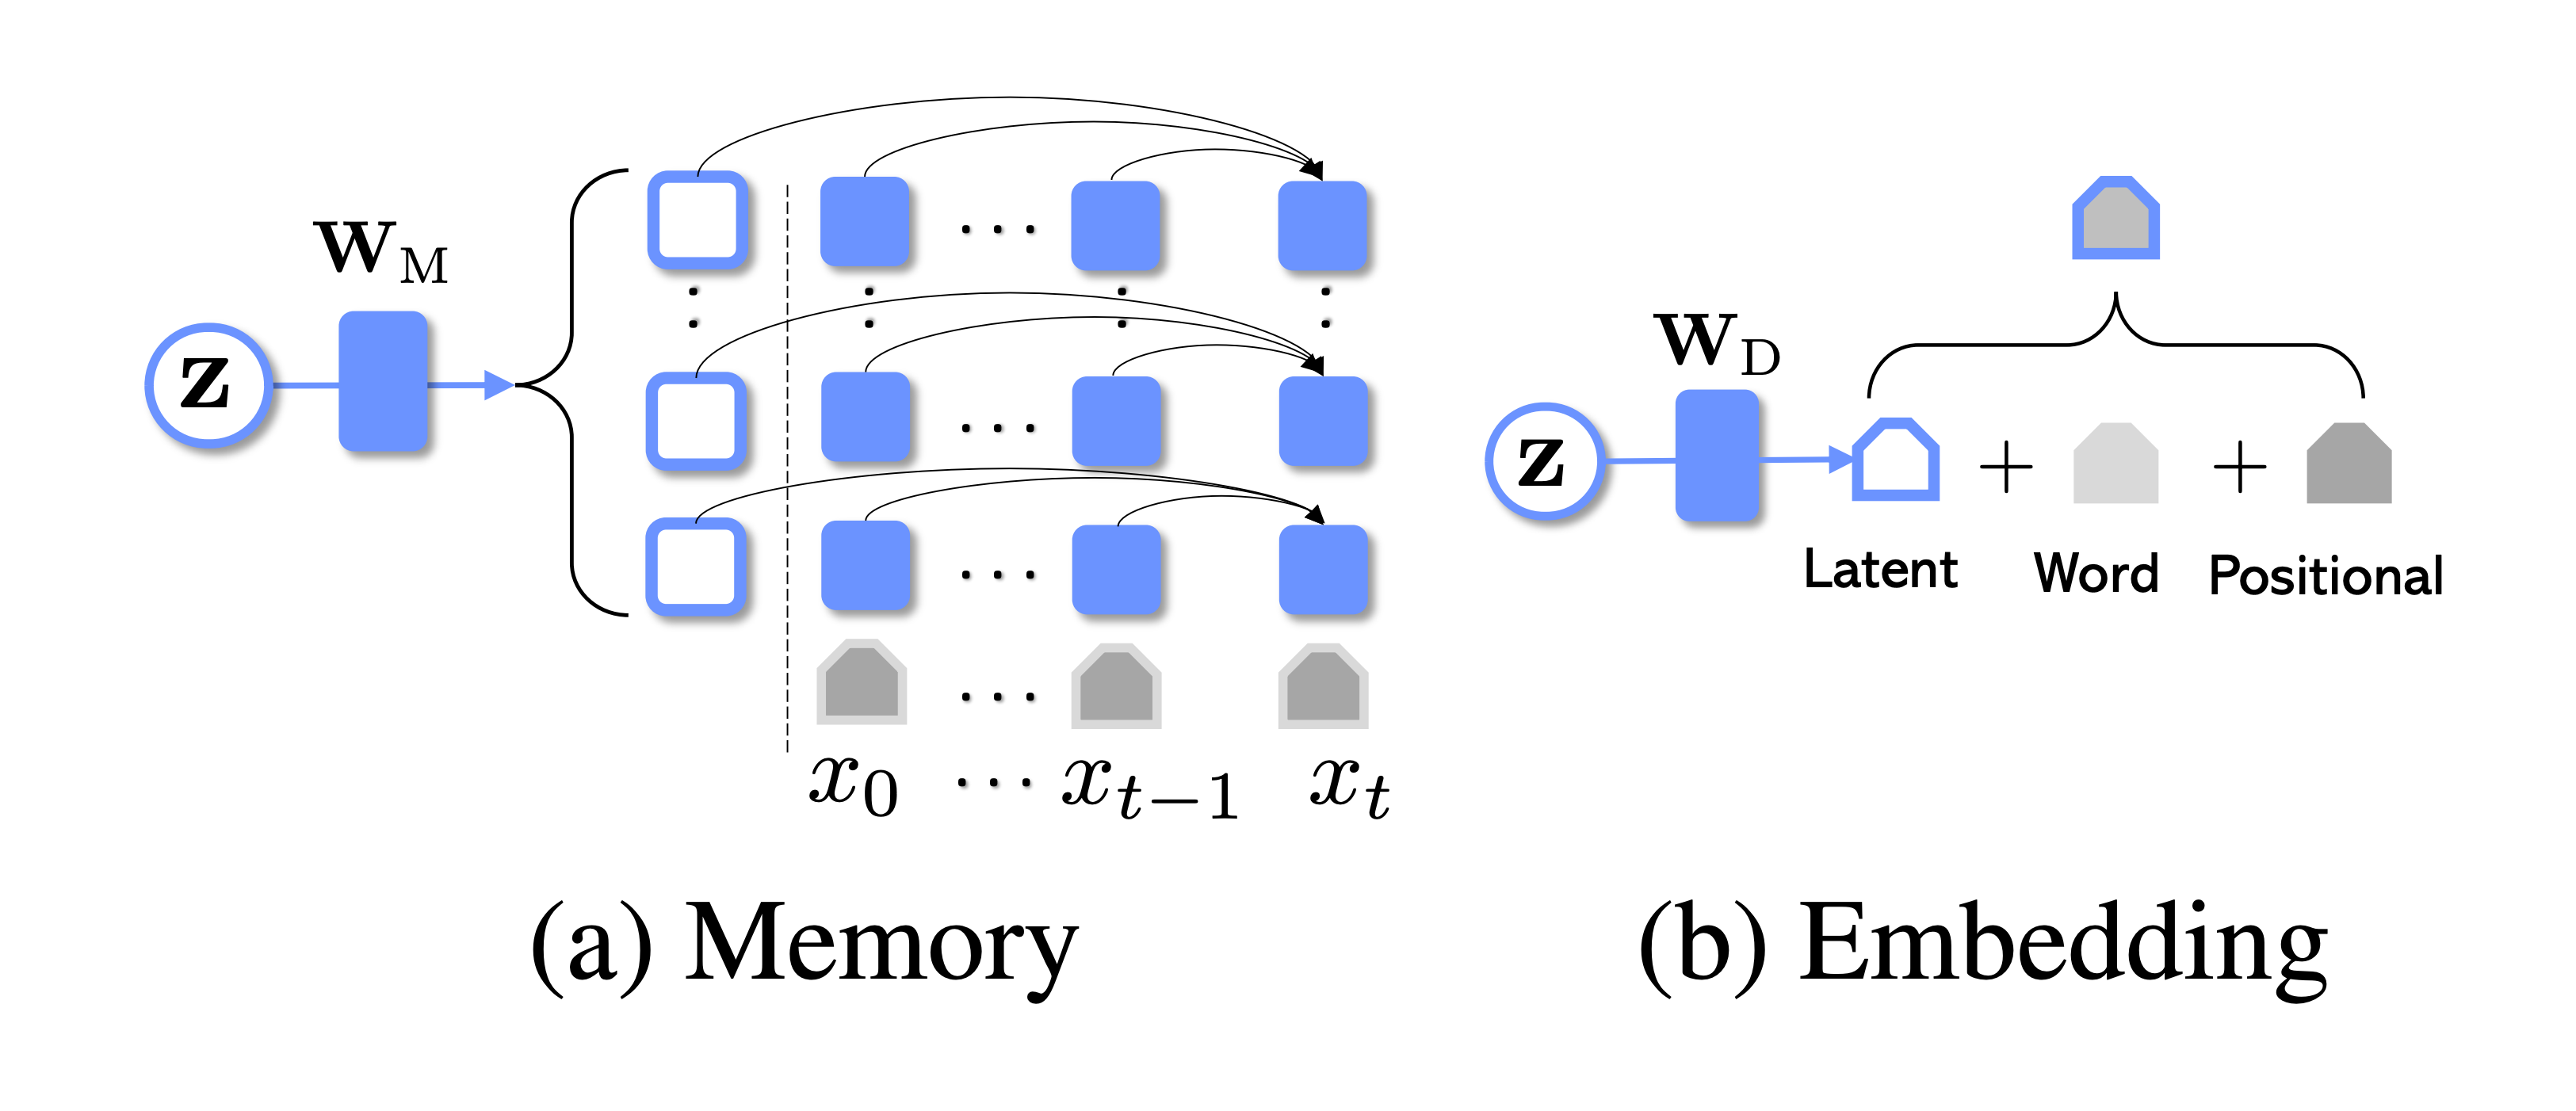
\includegraphics[width=11cm]{bilder/latent_optimus}
    \caption{Methoden, um den Latentvektor in GPT-2 zu injizieren \citep{DBLP:journals/corr/abs-2004-04092}}
    \label{latent_optimus}
\end{figure}

Um mit GPT-2 kontrolliert unter Verwendung des Latentvektors Text zu generieren, kann der Latentvektor entweder als Memoryvektor in die Past-Gewichtsmatrix injeziert oder auf die vorherigen Embeddings addiert werden \citep{DBLP:journals/corr/abs-2004-04092}.

Beim Embedding wird $z$ direkt auf den Embedding Layer addiert. Somit ergibt sich der neue Embedding Layer durch $h_{Emb}^{'} = h_{Emb} + W_D z$ mit der Gewichtsmatrix $W_D \in \mathbb{R}^{H \times P}$.
Der Decoder kann hier die zusätzlichen Informationen des Embeddings im Input und Output Layer verwenden.

Bei der Injezierung von $z$ als Memoryvektor $h_{Mem} \in \mathbb{R}^{L\times H}$ wird der Latentvektor in den Past-Key-Vektor von GPT-2 injeziert. 
Der Past-Key-Vektor beschleunigt normalerweise den Decodiervorgang von GPT-2, da bei einem Decodierungsdurchlauf zu den vorherigen Tokens bereits berechnete Key- und Valuevektoren der Attentionlayern gespeichert und wiederverwendet werden.
Diese Key-, Valuevektoren des Attentionlayers werden durch $h_{Mem} = W_M z$ mit $W_M \in \mathbb{R}^{LH \times P}$ ersetzt. GPT-2 kann so beim Decodieren auf den injezierten Latentvektor bei jeder Attentionberechnung zugreifen.

Die Parameter ${\phi_{BERT}, \theta_{GPT-2}, W_E,W_M,W_D}$ des VAEs werden mittels Cyclical Annealing Schedule \citep{cyc_anneal} trainiert, um das KL Vanishing Problem beim Trainieren eines VAEs zu verhindern.
Die $\beta$ Variable, die wie in Abschnitt \ref{cyc_anneal} dargestellt den KL-Regularisierungs Anteil steuert, wird für einen Trainingsdurchlauf für die erste halbe Menge der Trainingsdaten auf $\beta = 0$ gesetzt. Somit wird zu Beginn lediglich ein Autoencoder trainiert. 
Anschließend wird $\beta$ für das nächste Viertel der Trainingsmenge schrittweise von 0 auf 1 erhöht und für das letzte Viertel der Trainingsmenge auf 1 belassen, um das VAE Modell zu trainieren.

Insgesamt zeigt Optimus gute Ergebnisse in den Bereichen des Language Modeling, der kontrollierten Text Generation und des Language Understanding.


%%%%PAST KEY VEKTOR MATRIX == Vergangenheitsmatrix

\pagebreak
\subsection{\textsc{BiMeanVAE}}
\textsc{BiMeanVAE} ist ein von \citep{coop} vorgestelltes Modell, bestehend aus einem bidirektionalem LSTM Encoder und einem LSTM Decoder. 
Die Hiddensize der einzelnen LSTMs beträgt 512. Nach dem BiLSTM Encoder wird ein Mean Pooling Layer verwendet, um einen Latentvektor $z$ zu erhalten.
\textsc{BiMeanVAE} verwendet die Standard Variational Autoencoder Ziele, dass Minimieren des Rekonstruktionsfehlers mit KL-Regularisierung.
Die verwendete Prior Verteilung $p_\theta(z)$ ist die Gausssche Normalverteilung $\mathcal{N}(0,\mathcal{I})$. 
Beim Training wird ebenfalls das in Abschnitt \ref{cyc_anneal} beschriebene Cyclical Annealing Verfahren verwendet, um graduell vom Autoencoder zum Variational Autoencoder Trainingsziel überzuleiten.


\subsection{Latent Space Operationen}
VAEs erlernen bidirektionale Abbildungen zwischen dem Datenraum und ihrem Latentspace. 
Im Latentspace werden Eingabesequenzen von Optimus und \textsc{BiMeanVAE} jeweils durch einen Latentvektor dargestellt.
Die zur Generation verwendeten Latentvektoren können durch arithmetische Operationen verändert werden, wodurch sich die gesampelte Ausgabe des VAEs gezielt verändern und steuern lässt.

Durch die KL-Regularisierung beim Training von VAEs entsteht ein kontinuierlicher Latentspace, wodurch semantisch ähnliche Inhalte im Latentspace nah beieinander organisiert werden.
Somit kann zwischen mehreren Datenobjekten im Latentspace interpoliert werden.

Insbesondere für das kontrollierte Generieren von Bewertungen sind diese Latent Space Operationen, die VAEs ermöglichen, elementar.
So kann zum Beispiel zwischen mehreren Bewertungen interpoliert werden, um eine durchschnittliche Meinung zu generieren.

Sei zum Beispiel $\mathcal{Z}$ die Menge der encodierten Bewertungen zu einer Produktgruppe, so lässt sich aus einer Untergruppe der Vektoren $\mathcal{Z}^{'} \subseteq \mathcal{Z}$ durch Kombinieren eine gute Durchschnittsrepräsentation im Latentvektorraum finden.
Das genaue Vorgehen zum Finden einer solchen Untergruppe wird in Abschnitt \ref{coop_chap} beschrieben
\pagebreak
